\documentclass[a4paper]{article}
\setlength{\topmargin}{-1.0in}
\setlength{\oddsidemargin}{-0.2in}
\setlength{\evensidemargin}{0in}
\setlength{\textheight}{10.5in}
\setlength{\textwidth}{6.5in}
\usepackage{enumitem}
\usepackage{listings}
\usepackage{amsmath}
\usepackage{hyperref}
\usepackage{amssymb}
\usepackage{tikz}
\usepackage{graphicx}
\usetikzlibrary{automata, positioning, arrows.meta}
\usepackage{xcolor}
\definecolor{YellowOrange}{RGB}{255,174,66}

\hbadness=10000

\hypersetup{
    colorlinks=true,
    linkcolor=blue,
    filecolor=magenta,      
    urlcolor=cyan,
    pdftitle={Assignment 6},
    pdfpagemode=FullScreen,
    }
\def\endproofmark{$\Box$}
\newenvironment{proof}{\par{\bf Proof}:}{\endproofmark\smallskip}
\begin{document}
\begin{center}
{\large \bf \color{red}  Department of Computer Science} \\
{\large \bf \color{red}  Ashoka University} \\

\vspace{0.1in}

{\large \bf \color{blue}  Discrete Mathematics: CS-1104-1 \& CS-1104-2}

\vspace{0.05in}

    { \bf \color{YellowOrange} Assignment 6}
\end{center}
\medskip

{\textbf{Collaborators:} None} \hfill {\textbf{Name: Rushil Gupta} }

\bigskip
\hrule


\section{Straightforward}
    \begin{enumerate}
        \item \begin{enumerate}
            \item \begin{enumerate}
                \item abc
                \begin{itemize}
                    \item G1: $S \rightarrow aS \rightarrow abA \rightarrow abcA \rightarrow abc$
                    \item G2: $S \rightarrow A \rightarrow aA \rightarrow aB \rightarrow abC \rightarrow abcC \rightarrow abc$ \\
                \end{itemize}
                
                \item aabccc
                \begin{itemize}
                    \item G1: $S \rightarrow aS \rightarrow aaS \rightarrow aabA \rightarrow aabcA \rightarrow aabccA \rightarrow aabcccA \rightarrow aabccc$
                    \item G2: $S \rightarrow A \rightarrow aA \rightarrow aaA \rightarrow aabC \rightarrow aabcC \rightarrow aabccC \rightarrow aabcccC \rightarrow aabccc$ \\
                \end{itemize}

                \item aacc
                \begin{itemize}
                    \item G1: not possible, since we cannot transition from $S$ to $A$ without a $b$
                    \item G2: not possible, since we cannot transition from $B$ to $C$ without a $b$ \\
                \end{itemize}

                \item abbc
                \begin{itemize}
                    \item G1: not possible, since we cannot have two consequent $b$'s (the only way to get a $b$ is by transitioning from $S$ to $bA$, and after state $A$, we cannot add more $b$'s)
                    \item G2: not possible, since we cannot have two consequent $b$'s (the only way to get a $b$ is by transitioning from $B$ to $bC$, and after state $C$, we cannot add more $b$'s) \\ \\
                \end{itemize}
            \end{enumerate}

            \item G1 is regular because it is a right-linear grammar. Each production in G1 has a non-terminal on the left hand side and a terminal or a terminal followed by a non-terminal on the right hand side. \\
            
            G2 is not regular because it is not a right-linear grammar. The production $S \rightarrow A$ is not a right-linear production because it has a non-terminal on the left hand side and a non-terminal on the right hand side. \\ \\

            \item Consider the general form of the strings generated by G1:\\
            $S \rightarrow aS \rightarrow aaS \rightarrow aa \dots aS \rightarrow a^nbA \rightarrow a^nbcA \rightarrow a^nbcc...cA \rightarrow a^nbc^m$ \\
            
            Consider the general form of the strings generated by G2:\\
            $S \rightarrow A \rightarrow aA \rightarrow aaA \rightarrow aa \dots aA \rightarrow a^nbC \rightarrow a^nbcC \rightarrow a^nbcc...cC \rightarrow a^nbc^m$ \\

            Since the strings generated by G1 and G2 are the same, $L(G1) = L(G2)$. \\

            \item Yes, $L(G2)$ is a regular language because it is recognized by a right-linear grammar. \\
        \end{enumerate}

        \newpage
        \item \begin{enumerate}
            \item Proof using counterexample: \\

            Assume that $L(G_l) = L(G_r)$. Trying to generate the string $aab$ using $G_r$ and $G_l$:
            \begin{itemize}
                \item $G_r$: $A \rightarrow aB \rightarrow aaB \rightarrow aabB \rightarrow aab$
                \item $G_l$: $A \rightarrow Ba \rightarrow Baa \rightarrow Baa \rightarrow \cdots$ (It's important to note that we cannot generate a string ending with $b$ using $G_l$)
            \end{itemize}

            So, $L(G_l) \neq L(G_r)$. \\ \\

            \item To convert a right-linear grammar $G_r = <T, N, S, P>$ to an equivalent left-linear grammar $G_l = <T, N, S, P'>$, we can follow the steps below:\\
            \begin{itemize}
                \item Draw a finite automaton for the right-linear grammar using the production rules given.
                \item Reverse the initial and final states of the finite automaton.
                \item Reverse the edges direction in the finite automaton.
                \item Construct the left-linear grammar by using the production rules of the finite automaton.
                \item The left-linear grammar is now equivalent to the right-linear grammar. \\
            \end{itemize}

            \item Consider the right-linear grammar $G_r = <T, N, S, P>$ where $T = \{a, b\}$, $N = \{A, B\}$, $S = A$, and $P = \{A \rightarrow aB, B \rightarrow aB | bB | \epsilon\}$. Here is the FA representing the grammar:\\ \\
            \begin{tikzpicture}
                \node[circle, draw] (A) at (0, 0) {$A$};
                \node[circle, draw] (B) at (2, 0) {$B$};
                \node[circle, draw] (C) at (4, 0) {$C$};
                \draw (A) -> node[above]{a} (B);
                \draw (B) edge[loop below] node{a, b} (B);
                \draw (B) -> node[above]{$\epsilon$} (C);
            \end{tikzpicture}

            Note that C is the final/accept state. \\ \\

            Now, we reverse the initial and final states of the FA and reverse the edges direction. The new FA is as follows:\\ \\
            \begin{tikzpicture}
                \node[circle, draw] (A) at (0, 0) {$A$};
                \node[circle, draw] (B) at (2, 0) {$B$};
                \node[circle, draw] (C) at (4, 0) {$C$};
                \draw (B) -> node[above]{a} (A);
                \draw (B) edge[loop below] node{a, b} (B);
                \draw (C) -> node[above]{$\epsilon$} (B);
            \end{tikzpicture}

            Here, A is the final/accept state. \\ \\

            Here we see that the FA is not deterministic. However, upon extracting the grammar from the FA, we get the left-linear grammar $G_l = <T, N, S, P'>$ where $T = \{a, b\}$, $N = \{A, B\}$, $S = A$, and $P' = \{A \rightarrow Ba, B \rightarrow Ba | Bb | \epsilon\}$. \\

            \item To prove the correctness of the process, we need to show that $L(G_l) = L(G_r)$. \\
            Clearly, from the FA, we can see that the strings generated by $G_l$ are the same as the strings generated by $G_r$. \\

            So, $L(G_l) = L(G_r)$. \\
        \end{enumerate}

        \newpage
        % Let Σ = {a, b}. Consider the following regular grammars over Σ. L = {w = w1w2 · · · wn | (w1 = wn ∧ |w| ≡ 0 (mod 2)) ∨ (w1 ̸= wn ∧ |w| ≡ 1 (mod 2)), n > 0} 1 • Ls = {w = w1w2 · · · wn | w1 = wn, n > 0} • Ld = {w = w1w2 · · · wn | w1 ̸= wn n > 0} • Le = {w = w1w2 · · · wn | |w| ≡ 0 (mod 2), n > 0} • Lo = {w = w1w2 · · · wn | |w| ≡ 1 (mod 2), n > 0}
        \item \begin{enumerate}
            \item The DFA $M$ for $L$ is as follows: \\
            \begin{tikzpicture}[>={Stealth[inset=0pt,length=8pt,angle'=35,round]}, 
                shorten >=1pt, 
                auto,
                node distance=2.5cm, 
                semithick,
                initial text=$ $,
                state/.style={circle, minimum size=0.5cm, draw=black, very thick, fill=blue!20},
                accepting/.style={double distance=1.5pt, outer sep=1pt+1.5pt}
                ]
            
                % Nodes
                \node[initial,state] (q0) {$q_0$};
                \node[state] (q_odd_a) [above right=of q0] {$q_{odd}^a$};
                \node[state] (q_odd_b) [below right=of q0] {$q_{odd}^b$};
                \node[state,accepting] (q_even_aa) [right=of q_odd_a] {$q_{even}^{aa}$};
                \node[state,accepting] (q_even_bb) [right=of q_odd_b] {$q_{even}^{bb}$};
                \node[state] (q_even_ab) [above right=of q_even_aa] {$q_{even}^{ab}$};
                \node[state] (q_even_ba) [below right=of q_even_bb] {$q_{even}^{ba}$};
            
                % Paths
                \path[->]
                (q0) edge node [sloped, above] {a} (q_odd_a)
                     edge node [sloped, below] {b} (q_odd_b)
                (q_odd_a) edge [bend left=15] node {a} (q_even_aa)
                          edge [bend right=15] node {b} (q_even_ab)
                (q_odd_b) edge [bend right=15] node [swap] {a} (q_even_ba)
                          edge [bend left=15] node [swap] {b} (q_even_bb)
                (q_even_aa) edge [loop right] node {a} ()
                            edge [bend left=15] node [swap] {b} (q_odd_b)
                (q_even_bb) edge [loop right] node {b} ()
                            edge [bend right=15] node [swap] {a} (q_odd_a)
                (q_even_ab) edge [bend right=15] node [swap] {a} (q_odd_a)
                            edge [loop right] node {b} ()
                (q_even_ba) edge [loop right] node {a} ()
                            edge [bend right=15] node {b} (q_odd_b);
            \end{tikzpicture}

            % Design DFAs Ms, Md, Me, Mo for Ls, Ld, Le, Lo respectively.
            \item The DFA $M_s$ for $L_s$ is as follows: \\
            \begin{tikzpicture}[>={Stealth[inset=0pt,length=8pt,angle'=35,round]}, 
                shorten >=1pt, auto, node distance=3cm, semithick, initial text=$ $]
            
                \node[initial,state] (q0) {$q_0$};
                \node[state, accepting] (qa) [above right of=q0] {$q_a$};
                \node[state, accepting] (qb) [below right of=q0] {$q_b$};
                \node[state] (qao) [right of=qa] {$q_{a\_other}$};
                \node[state] (qbo) [right of=qb] {$q_{b\_other}$};
            
                \path[->]
                (q0) edge node {a} (qa)
                     edge node {b} (qb)
                (qa) edge [loop above] node {a} ()
                     edge [bend left] node {b} (qao)
                (qb) edge [loop below] node {b} ()
                     edge [bend right] node {a} (qbo)
                (qao) edge [bend left] node {a} (qa)
                      edge [loop right] node {b} ()
                (qbo) edge [bend right] node {b} (qb)
                      edge [loop right] node {a} ();
            \end{tikzpicture}

            \newpage
            The DFA $M_d$ for $L_d$ is as follows: \\
            \begin{tikzpicture}[>={Stealth[inset=0pt,length=8pt,angle'=35,round]}, 
                shorten >=1pt, auto, node distance=3cm, semithick, initial text=$ $]
            
                \node[initial,state] (q0) {$q_0$};
                \node[state] (qa) [above right of=q0] {$q_a$};
                \node[state] (qb) [below right of=q0] {$q_b$};
                \node[state, accepting] (qao) [right of=qa] {$q_{a\_other}$};
                \node[state, accepting] (qbo) [right of=qb] {$q_{b\_other}$};
            
                \path[->]
                (q0) edge node {a} (qa)
                     edge node {b} (qb)
                (qa) edge [loop above] node {a} ()
                     edge [bend left] node {b} (qao)
                (qb) edge [loop below] node {b} ()
                     edge [bend right] node {a} (qbo)
                (qao) edge [bend left] node {a} (qa)
                      edge [loop right] node {b} ()
                (qbo) edge [bend right] node {b} (qb)
                      edge [loop right] node {a} ();
            
            \end{tikzpicture} \\ \\

            The DFA $M_e$ for $L_e$ is as follows: \\
            \begin{tikzpicture}[>={Stealth[inset=0pt,length=8pt,angle'=35,round]}, 
                shorten >=1pt, auto, node distance=2cm, semithick, initial text=$ $]
            
                \node[initial,state,accepting] (qe) {$q_0$};
                \node[state] (qo) [right of=qe] {$q_1$};
            
                \path[->]
                (qe) edge [bend left] node {a,b} (qo)
                (qo) edge [bend left] node {a,b} (qe);
            
            \end{tikzpicture} \\ \\

            The DFA $M_o$ for $L_o$ is as follows: \\
            \begin{tikzpicture}[>={Stealth[inset=0pt,length=8pt,angle'=35,round]}, 
                shorten >=1pt, auto, node distance=2cm, semithick, initial text=$ $]
            
                \node[initial,state] (qe) {$q_0$};
                \node[state, accepting] (qo) [right of=qe] {$q_1$};
            
                \path[->]
                (qe) edge [bend left] node {a,b} (qo)
                (qo) edge [bend left] node {a,b} (qe);
            
            \end{tikzpicture} \\ \\ \\ \\

            \item To express the language $L$ in terms of $L_s$, $L_d$, $L_e$, and $L_o$, we should first understand how $L$ is defined and then see how it can be represented using the intersection and union of these four languages. The language $L$ is defined as:
            \[ L = \{ w = w_1 w_2 \ldots w_n \mid (w_1 = w_n \land |w| \equiv 0 \ (\text{mod}\ 2)) \lor (w_1 \neq w_n \land |w| \equiv 1 \ (\text{mod}\ 2)), n > 0 \} \]

            Breaking Down $L$: This definition can be split into two parts:
            \begin{enumerate}
                \item Strings where the first and last characters are the same, and the length of the string is even.
                \item Strings where the first and last characters are different, and the length of the string is odd.
            \end{enumerate}

            Given the languages:
            \begin{itemize}
                \item $L_s = \{ w \mid w_1 = w_n, n > 0 \}$ — Strings that start and end with the same character.
                \item $L_d = \{ w \mid w_1 \neq w_n, n > 0 \}$ — Strings that start and end with different characters.
                \item $L_e = \{ w \mid |w| \equiv 0 \ (\text{mod}\ 2), n > 0 \}$ — Strings of even length.
                \item $L_o = \{ w \mid |w| \equiv 1 \ (\text{mod}\ 2), n > 0 \}$ — Strings of odd length.
            \end{itemize}

            Expression Using Set Operations: We can now use set operations (intersection and union) to express $L$:
            \[ L = (L_s \cap L_e) \cup (L_d \cap L_o) \]

            \newpage
            \item Here is the NFA $N$ for $L$ using the relationship we found earlier: \\
            \begin{tikzpicture}[>={Stealth[inset=0pt,length=8pt,angle'=35,round]}, 
                shorten >=1pt, auto, node distance=4cm, semithick, initial text=$ $]
            
                % Define the style for the states
                \tikzset{state/.style={circle, draw, minimum size=1cm}}
            
                % Nodes
                \node[initial,state] (start) {$q_{start}$};
                \node[state, above right of=start, yshift=-1cm] (se) {$s_e$}; % Represents (L_s ∩ L_e)
                \node[state, below right of=start, yshift=1cm] (do) {$d_o$}; % Represents (L_d ∩ L_o)
                \node[state, accepting, right of=se, xshift=1cm] (acc1) {Accept};
                \node[state, accepting, right of=do, xshift=1cm] (acc2) {Accept};
            
                % Paths
                \path[->]
                (start) edge node [sloped, anchor=center, above] {$\epsilon$} (se)
                    edge node [sloped, anchor=center, below] {$\epsilon$} (do)
                (se) edge node [above] {on $L_s \cap L_e$ conditions} (acc1)
                (do) edge node [below] {on $L_d \cap L_o$ conditions} (acc2);
            \end{tikzpicture} \\ \\

            \newpage
            \item To prove that $L(M) = L(N) = L$, where $M$ is the DFA for the language $L$ and $N$ is the NFA constructed to represent $L$, we need to first describe the conditions defined by $L$ and then show how both automata satisfy these conditions. \\

            \textbf{Language $L$ Description:}
            \[ L = \{ w = w_1w_2 \ldots w_n \mid (w_1 = w_n \land |w| \equiv 0 \ (\text{mod}\ 2)) \lor (w_1 \neq w_n \land |w| \equiv 1 \ (\text{mod}\ 2)), n > 0 \} \]

            This language consists of strings where:
            \begin{enumerate}
                \item The first and last characters are the same, and the length of the string is even.
                \item The first and last characters are different, and the length of the string is odd. \\
            \end{enumerate}

            \textbf{Breaking Down into Sublanguages:}
            We defined the sublanguages as:
            \begin{itemize}
                \item $L_s = \{ w \mid w_1 = w_n, n > 0 \}$
                \item $L_d = \{ w \mid w_1 \neq w_n, n > 0 \}$
                \item $L_e = \{ w \mid |w| \equiv 0 \ (\text{mod}\ 2), n > 0 \}$
                \item $L_o = \{ w \mid |w| \equiv 1 \ (\text{mod}\ 2), n > 0 \}$ \\
            \end{itemize}

            We then express $L$ as:
            \[ L = (L_s \cap L_e) \cup (L_d \cap L_o) \]

            \textbf{Proof for $M$ (DFA):}
            \begin{itemize}
                \item We designed $M$ with the understanding that it needs to recognize strings that fit one of the two conditions:
                \begin{enumerate}
                    \item First and last characters the same, even length.
                    \item First and last characters different, odd length. \\
                \end{enumerate}
                \item The DFA $M$ was implicitly defined by combining the rules of $L_s$ and $L_e$ or $L_d$ and $L_o$ through specific states that track:
                \begin{enumerate}
                    \item The start character to check if it matches the end character.
                    \item The length of the string to determine if it is odd or even. \\
                \end{enumerate}
                \item Transitions in $M$ ensure that if a string starts with a character, say 'a', it keeps track of this 'a' and whether the subsequent length is odd or even, thereby determining which part of the language it satisfies. \\
            \end{itemize}

            \textbf{Proof for $N$ (NFA):}
            \begin{itemize}
                \item $N$ was constructed using $\epsilon$-transitions to start either the simulation of $(L_s \cap L_e)$ or $(L_d \cap L_o)$.
                \item The paths $(L_s \cap L_e)$ and $(L_d \cap L_o)$ in $N$ are independent and explicitly model the criteria set by these combinations.
                \item By using $\epsilon$-transitions, $N$ non-deterministically chooses to evaluate a string under one of the two required conditions, thus covering all elements of $L$. \\
            \end{itemize}

            \textbf{Equality:}
            \begin{itemize}
                \item $L(M)$ captures all strings as per the definition of $L$ since the DFA $M$ is constructed to switch states based on input while maintaining checks on start-end character equality/inequality and string length parity.
                \item $L(N)$ represents the same language $L$ by nondeterministically deciding which combination of sublanguages a given string belongs to, checking the conditions simultaneously in separate branches of the computation. Thus, both $M$ and $N$ correctly implement the logic required to accept exactly the strings defined in $L$, hence $L(M) = L(N) = L$. \\
            \end{itemize}
        \end{enumerate}


        \newpage
        % Here is the transcription of Question 4 from the image you uploaded: --- **4. Let Σ = {0, 1}, L is a given regular language over Σ, w_a ∈ L, and w_r ∉ L. You are free to choose w_a and w_r appropriately based on L such that |w_a| ≥ 5 and |w_r| ≥ 5 (you may need to choose shorter strings if the language does not accept / reject strings of length ≤ 5 and you may need to choose longer strings if the language does not accept / reject strings of length ≤ 5). State your choice.** **(a) Design an NFA N for L. Show the working of N for w_a and w_r.** **(b) Design a right linear regular grammar G for L. Show the derivation of w_a and w_r using G.** **(c) Prove: L = L(N) = L(G).** **Solve for the following languages:** - **L_I = {w = w_1w_2 · · · w_n | (w ≠ ε) ∧ (w_i = 0, i ≡ 0 (mod 2)), n > 0}** - **L_II = {w = w_1w_2 · · · w_n | |#{1}(w_1w_2 · · · w_i)| ≠ 0 (w_1w_2 · · · w_i)| ≤ 1, 1 ≤ i ≤ n}** - **L_III = {w = w_1w_2 · · · w_n | w_i-1w_iw_i+1 = 000 ∧ w_i-2 · · · w_i ≠ ∈ Λ w_i+2 · · · w_n ≠ ε, 3 ≤ i ≤ n - 2, n ≥ 5}** - **L_IV = {w = w_1w_2 · · · w_n | w_i^t ∈ {10, 110, 1110, 1111}, n ≥ 0}** **Note: When we write w = w_1w_2 · · · w_n, we mean w_i ∈ Σ and |w| = n ≥ 0 (unless specified otherwise).** --- This question provides an interesting challenge in designing NFAs, right linear grammars, and proving equivalences for various specified languages. If you need further assistance or specific solutions for any of the languages \(L_I\), \(L_II\), \(L_III\), or \(L_IV\), feel free to ask!
        % Let's tackle the tasks presented for the given languages \( L_I \), \( L_{II} \), \( L_{III} \), and \( L_{IV} \). We'll address each part of the question (designing an NFA, creating a grammar, and proving equality) sequentially for each language. ### Language \( L_I \) #### Description \( L_I = \{ w = w_1w_2 \cdot \cdot \cdot w_n \mid (w \neq \epsilon) \wedge (w_i = 0, i = 0 \ (\text{mod} \ 2)), n > 0 \} \) This language consists of non-empty strings where every character at an even index is a '0'. #### (a) Design an NFA \( N \) for \( L_I \) **States**: - \( q_0 \): Start state, accept odd indices. - \( q_1 \): Accepts '0' at even indices. **Transitions**: - \( q_0 \) reads '0' or '1' and moves to \( q_1 \). - \( q_1 \) reads '0' and moves back to \( q_0 \). **Accepting states**: - Both \( q_0 \) and \( q_1 \) could be accepting, as the string can be of any length as long as it conforms to the even-index rule. #### (b) Design a Right Linear Grammar \( G \) for \( L_I \) **Variables**: - \( S \): Start and intermediate state. - \( A \): Tracks accepting '0' at even indices. **Productions**: - \( S \rightarrow 0A \ | \ 1A \) - \( A \rightarrow 0S \ | \ \epsilon \) #### (c) Prove: \( L = L(N) = L(G) \) - **\( L(N) \) to \( L \)**: - By construction, \( N \) accepts all and only those strings where every even index character is '0'. The transitions enforce this rule, as \( q_1 \) only loops back to \( q_0 \) on a '0'. - **\( L(G) \) to \( L \)**: - The grammar generates a '0' or '1' from the start and then enforces a '0' at every next even position (through \( A \rightarrow 0S \)). This corresponds to the language definition. ### Application for \( L_I \) example: For \( w_a = "010101" \) and \( w_r = "1101" \): - \( w_a \) fits \( L_I \) as it obeys the even-index '0' rule. - \( w_r \) does not fit \( L_I \) as it has a '1' at the zeroth position. Now, let's briefly outline the method for the other languages, given the pattern provided: ### Language \( L_{II} \) This language includes strings where there is exactly one '1' in the string. #### (a) NFA Design for \( L_{II} \) You can design an NFA that starts in a state which transitions to an accepting state upon reading a '1' and rejects any further '1's while looping on '0's. #### (b) Right Linear Grammar for \( L_{II} \) - \( S \rightarrow 0S \ | \ 1A \) - \( A \rightarrow 0A \ | \ \epsilon \) #### (c) Prove \( L = L(N) = L(G) \) ### Language \( L_{III} \) This language includes strings where the substring "000" does not appear. #### (a) NFA Design for \( L_{III} \) Design an NFA that tracks up to two consecutive '0's but moves to a dead state upon the third consecutive '0'. #### (b) Right Linear Grammar for \( L_{III} \) - \( S \rightarrow 1S \ | \ 0A \ | \ \epsilon \) - \( A \rightarrow 1S \ | \ 0B \) - \( B \rightarrow 1S \ | \ \epsilon \) (no transition for '0' to prevent "000") #### (c) Prove \( L = L(N) = L(G) \) ### Language \( L_{IV} \) This language includes strings where no substring is one of {10, 110, 1110, 1111}. #### (a) NFA Design for \( L_{IV} \) Design an NFA that tracks these substrings and moves to a dead state upon matching any of them. #### (b) Right Linear Grammar for \( L_{IV} \) This might involve creating non-terminals for each forbidden sequence and ensuring transitions don't generate them. #### (c) Prove \( L = L(N) = L(G) \) This outline provides a framework for solving these kinds of problems. For detailed transitions and more complex proofs, you can apply the concepts of regular language manipulation using automata and grammars, ensuring the conditions stated for each language are met.
        \item \begin{enumerate}[label=\arabic*)]
            \item $L_I$:\\
            \begin{enumerate}[label=(\alph*)]
                \item The NFA $N$ for $L_I$ is as follows: \\
                \begin{tikzpicture}[>={Stealth[inset=0pt,length=8pt,angle'=35,round]}, 
                    shorten >=1pt, auto, node distance=3cm, semithick, initial text=$ $]
                
                    \node[initial,state] (q0) {$q_0$};
                    \node[state, accepting] (q1) [right of=q0] {$q_1$};
                
                    \path[->]
                    (q0) edge [loop above] node {1} ()
                         edge node {0} (q1)
                    (q1) edge [loop above] node {0} ()
                         edge node {1} (q0);
                \end{tikzpicture} \\

                \item The right linear grammar $G$ for $L_I$ is as follows: \\
                \begin{itemize}
                    \item Variables: $S, A$
                    \item Productions: $S \rightarrow 0A \ | \ 1A$ and $A \rightarrow 0S \ | \ \epsilon$
                \end{itemize}

                \item To prove $L = L(N) = L(G)$, we need to show that the strings generated by $N$ and $G$ are the same as the strings generated by $L$. \\
                \begin{itemize}
                    \item $L(N)$: The NFA $N$ accepts all strings where every character at an even index is a '0'.
                    \item $L(G)$: The right linear grammar $G$ generates strings where every character at an even index is a '0'. \\ \\
                \end{itemize}
            \end{enumerate}

            \item $L_{II}$:\\
            \begin{enumerate}[label=(\alph*)]
                \item The NFA $N$ for $L_{II}$ is as follows: \\
                \begin{tikzpicture}[>={Stealth[inset=0pt,length=8pt,angle'=35,round]}, 
                    shorten >=1pt, auto, node distance=3cm, semithick, initial text=$ $]
                
                    \node[initial,state] (q0) {$q_0$};
                    \node[state, accepting] (q1) [right of=q0] {$q_1$};
                
                    \path[->]
                    (q0) edge [loop above] node {0} ()
                         edge node {1} (q1)
                    (q1) edge [loop above] node {0} ()
                         edge [loop right] node {1} ();
                \end{tikzpicture} \\

                \item The right linear grammar $G$ for $L_{II}$ is as follows: \\
                \begin{itemize}
                    \item Variables: $S, A$
                    \item Productions: $S \rightarrow 0S \ | \ 1A$ and $A \rightarrow 0A \ | \ \epsilon$
                \end{itemize}

                \item To prove $L = L(N) = L(G)$, we need to show that the strings generated by $N$ and $G$ are the same as the strings generated by $L$. \\
                \begin{itemize}
                    \item $L(N)$: The NFA $N$ accepts all strings where there is exactly one '1'.
                    \item $L(G)$: The right linear grammar $G$ generates strings where there is exactly one '1'. \\ \\
                \end{itemize}
            \end{enumerate}

            \newpage
            \item $L_{III}$:\\
            \begin{enumerate}[label=(\alph*)]
                \item The NFA $N$ for $L_{III}$ is as follows: \\
                \begin{tikzpicture}[>={Stealth[inset=0pt,length=8pt,angle'=35,round]}, 
                    shorten >=1pt, auto, node distance=3cm, semithick, initial text=$ $]
                
                    \node[initial,state] (q0) {$q_0$};
                    \node[state] (q1) [right of=q0] {$q_1$};
                    \node[state] (q2) [right of=q1] {$q_2$};
                    \node[state] (q3) [right of=q2] {$q_3$};
                    \node[state] (q4) [right of=q3] {$q_4$};
                    \node[state, accepting] (q5) [right of=q4] {$q_5$};
                
                    \path[->]
                    (q0) edge node {0} (q1)
                    (q1) edge node {0} (q2)
                    (q2) edge node {0} (q3)
                    (q3) edge node {1} (q4)
                    (q4) edge node {0} (q5)
                    (q0) edge [loop above] node {1} ()
                    (q1) edge [loop above] node {1} ()
                    (q2) edge [loop above] node {1} ()
                    (q3) edge [loop above] node {1} ()
                    (q4) edge [loop above] node {1} ()
                    (q5) edge [loop above] node {0, 1} ();
                \end{tikzpicture} \\

                \item The right linear grammar $G$ for $L_{III}$ is as follows: \\
                \begin{itemize}
                    \item Variables: $S, A, B$
                    \item Productions: $S \rightarrow 1S \ | \ 0A \ | \ \epsilon$, $A \rightarrow 1S \ | \ 0B$, and $B \rightarrow 1S \ | \ \epsilon$
                \end{itemize}

                \item To prove $L = L(N) = L(G)$, we need to show that the strings generated by $N$ and $G$ are the same as the strings generated by $L$. \\
                \begin{itemize}
                    \item $L(N)$: The NFA $N$ accepts all strings where the substring "000" does not appear.
                    \item $L(G)$: The right linear grammar $G$ generates strings where the substring "000" does not appear. \\ \\
                \end{itemize}
            \end{enumerate}
        \end{enumerate}

    \end{enumerate}

\newpage
\section{$\neg$Straightforward}
    \begin{enumerate}
        \item a

    \end{enumerate}

\newpage
\section{Bonus}
    \begin{enumerate}[label=(\alph*)]
        \item Below is a table format describing the transitions for each state based on the corrected understanding of the diagram: \\
        \begin{center}
            \begin{tabular}{|c|c|c|}
                \hline
                \textbf{State} & \textbf{Reads 'a'} & \textbf{Reads 'b'} \\
                \hline
                $q_0$ & Goes to $q_2$ & Loops on $q_0$ \\
                $q_1$ & Goes to $q_0$ & Loops on $q_1$ \\
                $q_2$ & Goes to $q_3$ & Loops on $q_2$ \\
                $q_3$ & Goes to $q_1$ & Goes to $q_2$ \\
                \hline
            \end{tabular}
        \end{center}

        The table describes the transitions for each state based on the input read. \\ \\

        \item The regular grammar $G$ for the state machine $M$ is as follows: \\
        \begin{itemize}
            \item Variables: $S_0, S_1, S_2, S_3$
            \item Productions: $S_0 \rightarrow aS_2 \ | \ bS_0$, $S_1 \rightarrow aS_0 \ | \ bS_1$, $S_2 \rightarrow aS_3 \ | \ bS_2$, and $S_3 \rightarrow aS_1 \ | \ bS_2$ \\ \\
        \end{itemize}


        % Prove that L(G) = L(M).
        % To prove that the language generated by the grammar \( G \) (denoted \( L(G) \)) is equal to the language recognized by the automaton \( M \) (denoted \( L(M) \)), we need to establish two things: 1. **\( L(G) \subseteq L(M) \)**: Every string generated by grammar \( G \) is recognized by automaton \( M \). 2. **\( L(M) \subseteq L(G) \)**: Every string recognized by automaton \( M \) can be generated by grammar \( G \). ### Proving \( L(G) \subseteq L(M) \) We start by considering the production rules of \( G \) and how they correspond to transitions in \( M \). Each rule in \( G \) is derived directly from the transitions of \( M \): - \( S_0 \rightarrow aS_2 \,|\, bS_0 \) - \( S_1 \rightarrow aS_0 \,|\, bS_1 \) - \( S_2 \rightarrow aS_3 \,|\, bS_2 \) - \( S_3 \rightarrow aS_1 \,|\, bS_2 \) If a string \( w \) can be generated from a non-terminal \( S_i \) (corresponding to state \( q_i \) in \( M \)), then there exists a sequence of transitions in \( M \) starting from \( q_i \) that results in \( w \) being accepted if \( q_i \) leads to an accepting state after processing \( w \). Since the grammar's production rules mimic the state transitions: - Each production \( S_i \rightarrow aS_j \,|\, bS_k \) represents a valid transition \( q_i \) on 'a' to \( q_j \) and on 'b' to \( q_k \) in \( M \). - Thus, if \( w \) is generated by \( G \), starting from the start symbol corresponding to the initial state of \( M \), then following the transitions dictated by \( w \) in \( M \) must lead to an accepting state if \( w \) ends at a production that includes \( \epsilon \) or at a non-terminal that corresponds to an accepting state in \( M \). ### Proving \( L(M) \subseteq L(G) \) Conversely, consider any string \( w \) that is accepted by \( M \). Starting from the initial state \( q_0 \) (corresponding to the start symbol \( S_0 \)): - For every transition \( q_i \) to \( q_j \) on symbol \( x \) in \( M \), there is a corresponding production \( S_i \rightarrow xS_j \) in \( G \). - By following the path that \( M \) takes on \( w \), we can construct a derivation in \( G \) that generates \( w \), starting from \( S_0 \) and proceeding according to the symbols in \( w \). - If \( w \) ends in an accepting state in \( M \), the corresponding sequence of productions in \( G \) will either end in a non-terminal that generates \( \epsilon \) (if that state is considered accepting in \( G \)) or completes the generation of \( w \) without needing \( \epsilon \). ### Conclusion Because the transitions and productions match exactly, and the criteria for acceptance are mirrored between \( M \) and \( G \), it follows that every string in \( L(M) \) can be generated by \( G \) and vice versa. Hence, \( L(G) = L(M) \). This equivalence shows that the grammar \( G \) correctly models the automaton \( M \), both structurally and in terms of language recognition.
        \item To prove that $L(G) = L(M)$, we need to establish two things: \\
        \begin{enumerate}
            \item $L(G) \subseteq L(M)$: Every string generated by grammar $G$ is recognized by automaton $M$.
            \item $L(M) \subseteq L(G)$: Every string recognized by automaton $M$ can be generated by grammar $G$. \\
        \end{enumerate}

        \textbf{Proving $L(G) \subseteq L(M)$:} \\
        The production rules of $G$ correspond to the transitions in $M$. Each rule in $G$ is derived directly from the transitions of $M$. If a string $w$ can be generated from a non-terminal $S_i$ (corresponding to state $q_i$ in $M$), then there exists a sequence of transitions in $M$ starting from $q_i$ that results in $w$ being accepted if $q_i$ leads to an accepting state after processing $w$. Since the grammar's production rules mimic the state transitions, each production $S_i \rightarrow aS_j \ | \ bS_k$ represents a valid transition $q_i$ on 'a' to $q_j$ and on 'b' to $q_k$ in $M$. Thus, if $w$ is generated by $G$, starting from the start symbol corresponding to the initial state of $M$, then following the transitions dictated by $w$ in $M$ must lead to an accepting state if $w$ ends at a production that includes $\epsilon$ or at a non-terminal that corresponds to an accepting state in $M$. \\

        \textbf{Proving $L(M) \subseteq L(G)$:} \\
        Consider any string $w$ that is accepted by $M$. Starting from the initial state $q_0$ (corresponding to the start symbol $S_0$), for every transition $q_i$ to $q_j$ on symbol $x$ in $M$, there is a corresponding production $S_i \rightarrow xS_j$ in $G$. By following the path that $M$ takes on $w$, we can construct a derivation in $G$ that generates $w$, starting from $S_0$ and proceeding according to the symbols in $w$. If $w$ ends in an accepting state in $M$, the corresponding sequence of productions in $G$ will either end in a non-terminal that generates $\epsilon$ (if that state is considered accepting in $G$) or completes the generation of $w$ without needing $\epsilon$. \\

        \textbf{Conclusion:} \\
        Because the transitions and productions match exactly, and the criteria for acceptance are mirrored between $M$ and $G$, it follows that every string in $L(M)$ can be generated by $G$ and vice versa. Hence, $L(G) = L(M)$. This equivalence shows that the grammar $G$ correctly models the automaton $M$, both structurally and in terms of language recognition. \\
    \end{enumerate}

\end{document}